\documentclass[a4paper,12pt]{article}

% ----------------------------
% Pacchetti utili
% ----------------------------
\usepackage[utf8]{inputenc}
\usepackage[T1]{fontenc}
\usepackage[italian]{babel}
\usepackage{graphicx}
\usepackage{xcolor}
\usepackage{colortbl}
\usepackage{geometry}
\usepackage{setspace}
\usepackage{fancyhdr}
\usepackage{tikz}
\usepackage[colorlinks=true, linkcolor=blue, urlcolor=blue, citecolor=blue]{hyperref}
% ----------------------------
% Impostazioni pagina
% ----------------------------
\geometry{
    top=2cm,
    bottom=2cm,
    left=2cm,
    right=2cm
}

\setstretch{1.2}

% ----------------------------
% Dati personalizzabili
% ----------------------------
\newcommand{\Gruppo}{Atlas}
\newcommand{\Email}{\href{mailto:team9.atlas@gmail.com}{\textcolor{blue}{\underline{team9.atlas@gmail.com}}}}
\newcommand{\TitoloUno}{Dichiarazione degli impegni}
\newcommand{\DataModifica}{28/10/2025}
\newcommand{\LogoGruppo}{img/AtlasLogo.png} % Inserisci il file del logo

% --- Nuove variabili aggiunte ---
\newcommand{\VersioneDocumento}{v0.2} % <-- modifica qui la versione o ID
\newcommand{\Interno}{Interno} 

\pagestyle{fancy}
\fancyhf{}
\fancyhead[L]{\Gruppo}
\fancyhead[R]{Documento: \Interno \space - \space \DataModifica}
\fancyfoot[C]{\thepage}

% ----------------------------
% Inizio documento
% ----------------------------
\begin{document}

% ----------------------------
% Prima pagina
% ----------------------------
\begin{titlepage}
    \centering

    % Logo in alto
    \vspace*{0cm}
    \begin{tikzpicture}
        \clip (0,-0.1) circle (4.6cm); % raggio = metà della larghezza desiderata
        \node at (0,0) {\includegraphics[width=10cm]{\LogoGruppo}};
    \end{tikzpicture}\\[0.8cm]

    % Nome gruppo ed email sotto al logo
    {\LARGE \textbf{\Gruppo}}\\[0.1cm]
    {\large \Email}\\[1.2cm]

    % Sottotitolo del progetto
    {\Large \textit{Progetto di ingegneria del software A.A. 2025/2026}}\\[1.5cm]

    % Titolo principale
    {\Huge \textbf{\TitoloUno}}\\[.5cm]

    % Dati riunione
    \begin{tabular}{rl}
        \textbf{Data ultima modifica:} & \DataModifica \\
        \textbf{Versione:} & \VersioneDocumento \\
    \end{tabular}

\end{titlepage}


\section*{Tabella delle revisioni}{
    \begin{center} 
        \begin{tabular}{|l|l|l|l|l|}
            \hline
            \textbf{Versione} & \textbf{Data} & \textbf{Autore} & \textbf{Verificatore} & \textbf{Descrizione} \\
            \hline
            \VersioneDocumento & 2025/10/29 & Giacomo Giora & Francesco Marcolongo & Aggiunta contenuti \\
            \hline
            v0.1 & 2025/10/28 & Andrea Difino & & Prima Stesura \\
            \hline
        \end{tabular}
    \end{center}
}

\newpage

\tableofcontents

\newpage

\section{Introduzione}{
    In questo documento è presente il preventivo del progetto, la stima delle ore previste e la ripartizione di queste ultime tra i membri del gruppo, definiti in base a un ragionamento sui ruoli necessari a svolgere il progetto riguardante il capitolato \textbf{C1 - Automated EN18031 Compliance Verification} proposto dall'azienda \textbf{Bluewind S.r.l.}.
}

\section{Impegni Orari}{
    Ogni componente del gruppo \textit{Atlas} si impegna a dedicare 91 ore produttive per il progetto, ottenendo un monte ore totale di 637 ore. 
    \newline La seguente tabella illustra la divisione delle ore per ogni ruolo con relativi costi:
    \begin{center}
        \begin{tabular}{|l|c|c|c|c|c|}
            \hline
            \rowcolor{gray!20}
            \textbf{Ruolo} & \textbf{Costo/h (€)} & \textbf{Stima Ore} & \textbf{Ore/Membro} & \textbf{Costo (€)} & \textbf{\%} \\
            \hline
            Responsabile & 30 & 56 & 8 & 1680 & 8.8 \\
            \hline
            Amministratore & 20 & 70 & 10 & 1400 & 11.0 \\
            \hline
            Analista & 25 & 84 & 12 & 2100 & 13.2 \\
            \hline
            Progettista & 25 & 112 & 16 & 2800 & 17.5 \\
            \hline
            Verificatore & 15 & 168 & 24 & 2520 & 26.4 \\
            \hline
            Programmatore & 15 & 147 & 21 & 2205 & 23.1 \\
            \hline
            \rowcolor{gray!20}
            \multicolumn{2}{|c|}{\textbf{Totale}} & \textbf{637} & \textbf{91} & \textbf{12705} & \textbf{100} \\
            \hline
        \end{tabular}

        \begin{figure}[h]
            \centering
            \begin{tikzpicture}
                \node at (0,0) {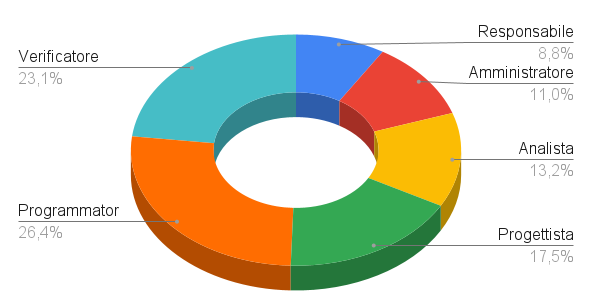
\includegraphics[width=15cm]{img/SuddivisioneRuoli.png}};
            \end{tikzpicture}
            \caption{Suddivisione ruoli}
            \label{fig:suddivisione-ruoli}
        \end{figure}
    \end{center}
}

\newpage
\section{Ruoli e motivazioni delle ore dedicate}{
    \subsection{Funzione ruoli}{
        Il calcolo del monte ore per ruolo è avvenuto tenendo in considerazione le seguenti funzioni per i ruoli da ricoprire:
        
        \begin{itemize}
            \item \textbf{Responsabile}: Punto di riferimento per le comunicazioni con il committente. Deve riuscire ad anticipare l'evoluzione del progetto in modo da pianificare le attività, gestire il team e tenere sotto controllo i progressi. Ha responsabilità di scelta e approvazione, per cui è essenziale e partecipa per tutta la durata del progetto;
            \item \textbf{Amministratore}: Si occupa dell'efficienza e dell'operatività dell'ambiente di sviluppo, deve assicurarsi che in ogni istante le risorse siano presenti e operanti. Ha il compito di gestione del controllo della configurazione del prodotto, del versionamento e della documentazione di progetto e definisce procedure, strumenti e convenzioni;
            \item \textbf{Analista}: Si occupa di capire e formalizzare il problema in maniera chiara. Il suo lavoro ha grande impatto sulla riuscita del progetto, in quanto raccoglie i requisiti dal cliente, li analizza e li specifica in modo chiaro e verificabile;
            \item \textbf{Progettista}: Si occupa dello sviluppo della soluzione al problema presentato tramite le attività di progettazione. Traduce i requisiti in architettura e soluzioni tecniche, definisce la struttura del sistema e sceglie tecnologie, pattern, protocolli di comunicazione;
            \item \textbf{Programmatore}: Si occupa di implementare la soluzione trovata dal progettista in codice, realizzando concretamente il software, e di contribuire ai test unitari di ausilio alla verifica;
            \item \textbf{Verificatore}: Deve essere a conoscenza delle norme e deve avere capacità di giudizio e relazione con il codice sorgente in particolare e con il sistema in generale. Si occupa di attività di verifica e validazione, partecipando all'intero ciclo di vita e controllando che il prodotto rispetti i requisiti e sia di qualità attraverso i test;
        \end{itemize}
    }
    
    \subsection{Distribuzione ore}{
        La distribuzione delle ore tra i vari ruoli è stata definita in funzione delle responsabilità specifiche e delle necessità progettuali relative al capitolato \textbf{C1 - Automated EN18031 Compliance Verification}.
        \vspace{0.3cm}
        \newline
        La figura del responsabile non è coinvolta in tutte le attività operative, infatti il suo ruolo è principalmente di coordinamento, pianificazione e controllo. Con 56 ore, dedicherà il tempo a definire piani, supervisionare l'avanzamento e approvare le consegne.
        \vspace{0.3cm}
        \newline
        L'amministratore deve impostare l'ambiente di lavoro e mantenerlo efficiente per tutto il progetto. Avendo un ruolo tecnico-organizzativo, le sue attività saranno periodiche ma non costanti: intense all'inizio e in corrispondenza dei rilasci, per un totale di 70 ore. Centrale sarà la definizione di un way of working appropriato per il team nelle fasi iniziali.
        \vspace{0.3cm}
        \newline
        La figura dell'analista deve invece impiegare tempo significativo, in particolare nella fase iniziale, per l'analisi dei requisiti, che richiede confronto con il committente e formalizzazione accurata, portando il suo monte ore a 84. Questa valutazione si basa anche sul fatto che il capitolato lascia ampi margini di libertà nella scelta delle tecnologie e nella progettazione del software (e dunque è necessaria un'analisi opportuna).
        \vspace{0.3cm}
        \newline
        Il progettista, con 112 ore, richiede tempo per la traduzione dei requisiti e la produzione di scelte tecnologiche efficaci (come i design pattern), ed è quindi una fase complessa che richiede precisione e revisione continua.
        \vspace{0.3cm}
        \newline
        Il programmatore con una stima di 147 ore, costituisce la parte sostanziale del lavoro di implementazione del prodotto, richiedendo tempo per implementare e correggere funzionalità.
        \vspace{0.3cm}
        \newline
        Il verificatore infine, con 168 ore, è la voce con più ore in assoluto, essendo necessario in tutte le fasi di progetto per garantire la qualità del prodotto attraverso test accurati. Anche in questo caso il monte ore assegnato è motivato dalle esigenze progettuali: testare il funzionamento dei vari decision tree (passo per passo) per valutare la conformità con gli standard di sicurezza di diversi dispositivi rappresenta sicuramente un compito oneroso e dispendioso in termini di tempo.
        \vspace{0.3cm}
        \newline
        In conclusione, questa distribuzione mira a bilanciare le esigenze del progetto, essendo esso complesso dal punto di vista dell'analisi e della verifica, e garantendo che ogni ruolo abbia il tempo necessario per adempiere alle proprie responsabilità in modo efficace.
    }
}

\section{Rotazione dei ruoli}{
    Le ore di lavoro verranno suddivise equamente tra i membri del gruppo, in modo da garantire che ciascuno possa ricoprire tutti i ruoli nel corso del progetto. È previsto un periodo di assegnazione del ruolo di due settimane, al termine del quale avverrà una rotazione e ciascun membro assumerà un ruolo diverso rispetto a quello svolto in precedenza, rispettando i vincoli di progetto. In questo modo, ogni membro del gruppo avrà l'opportunità di acquisire esperienza in ogni fase di ciclo di vita del software, migliorando le proprie competenze e contribuendo in modo più completo al successo del progetto, oltre che di valutarsi nello svolgimento dei vari ruoli.
}

\section{Preventivo e stima di consegna}{
    A seguito delle valutazioni del gruppo Atlas, l'impegno orario totale è di nr. 637 ore, il preventivo calcolato relativo al capitolato \textit{C1 - Automated EN18031 Compliance Verification} equivale a \textbf{12705€} e la scadenza stiamata di consegna è prevista entro e non oltre la data \textbf{2026-03-20}.
}

\end{document}